\documentclass[a4paper]{scrartcl}
\usepackage[ngerman]{babel}
\usepackage[utf8]{inputenc}
\usepackage{amssymb,amsmath}
\usepackage{graphicx}
\usepackage[inline]{enumitem}
\setlist{noitemsep}
\usepackage[binary-units=true]{siunitx}
\usepackage{hyperref}
\usepackage{parskip}
\usepackage[nameinlink,noabbrev,ngerman]{cleveref} % has to be after hyperref
\usepackage{nicefrac}  % for \nicefrac{1}{3}
\usepackage{csquotes}  % for \enquote{what you want to quote}
\usepackage{booktabs}  % for \toprule, \midrule and \bottomrule
\usepackage{minted} % needed for the inclusion of source code
\usepackage{mdframed}
\usepackage{mathtools}
\usepackage{tikz}
\usetikzlibrary{calc}

% for \begin{enumerate}[label=(\Alph*)], see http://tex.stackexchange.com/a/129960/5645
\usepackage{enumitem}

\setcounter{secnumdepth}{2}
\setcounter{tocdepth}{2}

\usepackage{wasysym}  % For \CheckedBox
\usepackage{microtype}

\newcommand\DrawControl[3]{
  node[#2,circle,fill=#2,inner sep=2pt,label={above:$#1$},label={[black]below:{\footnotesize#3}}] at #1 {}
}

\begin{document}
\selectlanguage{ngerman}
\title{2012 Nachklausur (WS 2011/12)}

\setcounter{section}{1}
%%%%%%%%%%%%%%%%%%%%%%%%%%%%%%%%%%%%%%%%%%%%%%%%%%%%%%%%%%%%%%%%%%%%%%%%%%%%%%
\section*{Aufgabe 1: Beleuchtung}
\subsection*{Teilaufgabe 1a}
\textit{Welche 4 Vektoren werden benötigt, um die reflektierte Farbe an einem Vertex bzw.
Oberflächenpunkt mit dem Phong-Beleuchtungsmodell zu berechnen? Illustrieren
Sie Ihre Antwort mit einer Skizze, die den Oberflächenpunkt, die Betrachter-
und die Lichtquellenposition beinhaltet.}

\begin{figure}[h]
    \centering
    \includegraphics*[width=0.8\linewidth, keepaspectratio]{1a.png}
    \caption{Whatever}
    \label{fig:1a}
\end{figure}

\begin{enumerate}
    \item Lichtvektor $L$
    \item Normale $N$
    \item View-Vektor $V$
    \item Reflektiertes Licht $R_L$
\end{enumerate}


\subsection*{Teilaufgabe 1b}
Beim Phong-Beleuchtungsmodell setzt sich das reflektierte Licht aus 3~Komponenten
zusammen: ambient, diffus und spekular.

\begin{mdframed}
Das Phong-Beleuchtungsmodell lautet:
\[I = \overbrace{k_a \cdot I_L}^{\text{ambient}}
    + \overbrace{k_d \cdot I_L \cdot (N \cdot L)}^{\text{diffus}}
    + \overbrace{k_s \cdot I_L \cdot (R_L \cdot V)^n}^{\text{spekular}}\]
\end{mdframed}

Erläutern Sie kurz, welche dieser Komponenten ihren Wert aus welchem Grund ändert
bzw. ändern, wenn:

\begin{itemize}
    \item \textit{der Vertex verschoben wird, aber die Lichtquelle- und
          Betrachterposition unverändert bleibt?}
          \begin{itemize}
              \item Spekular: $R_L$ und $V$ ändern sich
              \item Diffus: $L$ ändert sich
          \end{itemize}
    \item \textit{sich die Betrachterposition ändert, aber Lichtquelle und Vertex unverändert bleiben?}
          \begin{itemize}
              \item Spekular: $V$ ändert sich
          \end{itemize}
\end{itemize}

\subsection*{Teilaufgabe 1c}
\textit{Welche Aufgabe hat der Phong-Exponent? Welche Auswirkungen hat es, wenn sein
Wert größer bzw. kleiner gewählt wird?}
Imperfekte Spiegelung: Je größer der Phong-Exponent desto konzentrierter die Spiegelung, heißt der spekulare Lichtfleck wird kleiner aber dafür intensiver.

\subsection*{Teilaufgabe 1d}
\textit{Warum verbessert eine Unterteilung von Primitiven in kleinere die Darstellungsqualität, wenn Gouraud-Shading verwendet wird?}

Bei Gouraud-Shading wird die Farbe an den Vertices berechnet und dazwischen
interpoliert. Dadurch können Glanzlichter verloren gehen, die in der Mitte von
Primitiven liegen. Bei kleineren Primitiven ist die Wahrscheinlichkeit, dass
dies passiert geringer. Außerdem ergibt die Interpolation genauere Ergebnisse,
da die Vertices näher an den Punkten liegen, für die interpoliert wird

\section*{Aufgabe 2: Blending}
\subsection*{Teilaufgabe 2a}
\begin{enumerate}[label=(\Roman*)]
    \item
    \begin{itemize}
        \item Rot-Wert nach (1): $1$
        \item Rot-Wert nach (2): $\overbrace{0.5}^{\mathclap{\text{SRC\_ALPHA}}} \cdot \underbrace{1.0}_{\mathclap{\text{SRC\_COLOR}}} + \overbrace{(1-0.5)}^{\mathclap{\text{1-SRC\_ALPHA}}} \cdot \underbrace{0.2}_{\mathclap{\text{DST\_COLOR}}} = 0.6$\vspace{2.5pt}
        \item Rot-Wert nach (3): $0.5\cdot0.6+0.5\cdot0.4=0.5$
    \end{itemize}
    \item
    \begin{itemize}
        \item Rot-Wert nach (1): $1$
        \item Rot-Wert nach (2): $0.5\cdot1.0+0.5\cdot0.4=0.7$
        \item Rot-Wert nach (3): $0.5\cdot0.7+0.5\cdot0.2=0.45$
    \end{itemize}
    \item \textit{Welche Konsequenzen hat dies für das Zeichnen von sich
                  überlappenden semi-transparenten Objekten?}\\
          Erfordert Tiefensortierung. Im allgemeinen ist Blending nicht
          kommutativ.
\end{enumerate}

\subsection*{Teilaufgabe 2b}
\textit{Ein Zaun wird mit OpenGL gezeichnet, indem ein \texttt{GL\_QUAD}
-Primitiv mit einer Textur gezeichnet wird, die den Wert~1 enthält, wo sich
Lücken im Zaun befinden, und sonst den Wert 0 enthält. Warum sollte man in
diesem Fall Alpha-Testing statt Blending verwenden?}

Der Tiefenalgorithmus sieht nicht, dass der Zaun an manchen Stellen
durchsichtig ist und zeichnet deswegen Objekte die dahinter liegen nicht. Mit
Alpha-Testing werden dahinterliegende Objekte gezeichnet.

\subsection*{Teilaufgabe 2c}
\begin{itemize}
    \item Rufe \texttt{DrawScene} auf, Setze Source- und Destination-Faktor auf
          1/Anzahl Lichtquellen,
    \item verschiebe Lichtquelle,
    \item rufe \texttt{DrawScene} auf (Blending der Ergebnisse),
    \item setze Source auf 2/Anzahl,
    \item verschiebe Lichtquelle,
    \item rufe DrawScene auf (Blending der Ergebnisse),
    \item usw. bis alle Lichtquellen durch sind
\end{itemize}

\section*{Aufgabe 3: Texturierung}
\subsection*{Teilaufgabe 3a: Mip-Maps}
\begin{enumerate}[label=(\roman*)]
    \item \textit{Welches Problem löst Mip-Mapping?}\\
          Das Aliasing-Problem bei Minification.
    \item \textit{Was für Vorbereitungen werden für eine Textur getroffen?}\\
          Man berechnet Mipmap-Stufen, indem die Höhe und Breite der Textur
          jeweils halbiert wird.
    \item \textit{Wie erfolgt der Zugriff auf die Textur}?\\
          Texelgröße($n$) $\leq$ Größe des Pixelfootprints auf der Textur $<$ Texelgröße($n+1$)
\end{enumerate}

\subsection*{Teilaufgabe 3b: Environment-Maps}
\textit{Erläutern Sie kurz, wofür Environment-Mapping verwendet wird.}

Darstellung reflektierender Objekte mit Spiegelung von Umgebung ohne
geometrische Repräsentation.

\textit{Welche grundlegende Annahme wird dabei gemacht?}

Die Umgebung ist weit genug entfernt, sodass die Position keine Rolle spielt
und nur die Richtung genommen werden muss.

\subsection*{Teilaufgabe 3c}
\begin{tikzpicture}
\draw[->] (-0.5,0) -- (1.5,0);
\draw[->] (0,-0.5) -- (0,1.5);
\draw[fill=black] (0.5, 0) -- (1,0) -- (1,0.5) -- (0.5,0.5) -- cycle;
\draw[fill=black] (0,0.5) -- (0.5,0.5) -- (0.5,1) -- (0,1) -- cycle;
\draw (0,0) -- (1,0) -- (1,1) -- (0,1) -- cycle;
\end{tikzpicture}

\section*{Aufgabe 4: Hierarchische Datenstrukturen}
\subsection*{Teilaufgabe 4a}
 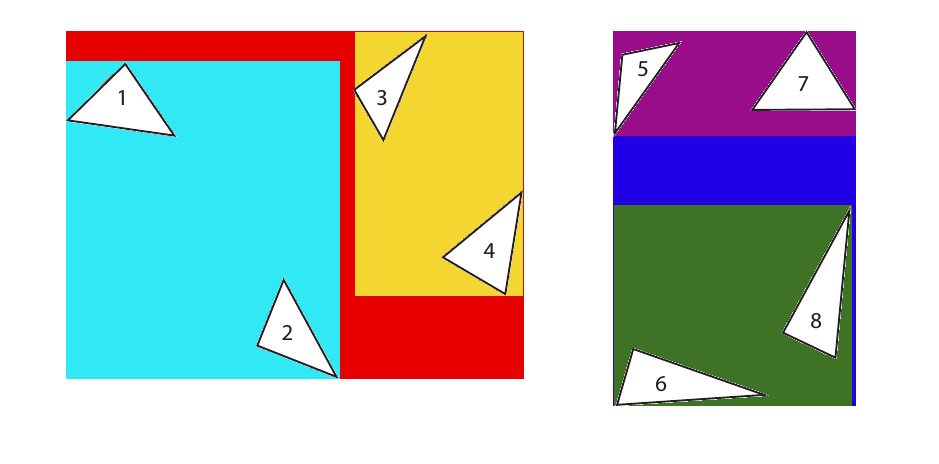
\includegraphics[scale=0.5]{BVH.png}

 \begin{tikzpicture}[level/.style={sibling distance=10em/#1},
  every node/.style = {shape=rectangle,
    draw, align=center}]]
  \node{}
    child { node[fill=red] {}
      child { node[fill=yellow] {}
          child { node {3} }
          child { node {4} } }
      child {node[fill=blue!50!green!40] {}
          child { node {1} }
          child { node {2}} }}
    child { node[fill=blue] {}
      child { node[fill=green!50!black] {}
        child { node[] {6} }
        child { node {8} } }
      child { node[fill=violet] {}
        child{ node {7} }
        child{node {5} }} };
 \end{tikzpicture}

\subsection*{Teilaufgabe 4b: SAH}
\textit{Welches Ziel verfolgt man beim Einsatz von Surface Area Heuristics (SAH)?}

Im Mittel sollen zufällige Strahlen, die den betrachteten Knoten schneiden, den
gleichen Aufwand verursachen, egal welcher Kindknoten traversiert wird (vgl.
Folie~90)

\textit{Erklären Sie kurz die Grundidee der SAH. Wie ändert sich die
Konstruktion eines kD-Baumes bei Anwendung dieser Technik?}

Die Wahrscheinlichkeit dafür dass man ein Primitiv trifft, wenn man die
Bounding Box getroffen hat, soll groß werden. Konstruktion bezieht
Kostenfunktion (Kosten für Schnitt mit Knoten) mit ein, damit die Kosten
minimiert werden. Surface Area der Primitive soll einen großen Anteil der
Bounding Box ausmachen.

\textit{Welche Größen fließen dabei zusätzlich mit ein?}
\begin{enumerate}[label=(\arabic*)]
    \item Primitiv-Flächeninhalt
    \item Surface Area der Box
    \item Kosten der Traversierung eines Knotens im Verhältnis zu Kosten eines Strahl-Primitiv-Tests
\end{enumerate}

\subsection*{Teilaufgabe 4c}
\textit{Warum ist das Object-Median -Kriterium meist nicht das performanteste
Unterteilungskriterium, wenn eine Bounding Volume Hierarchie beim Raytracing
einer statischen Szene eingesetzt werden soll?}

Suboptimal, wenn es Stellen gibt, an denen wenige Primitive liegen und welche
mit vielen Primitiven auf wenig Raum $\rightarrow$ es gib Boxen mit viel leerem
Raum drin.

\textit{In welchen Fällen ist das Object-Median-Kriterium nicht schlechter als
Surface Area Heuristics?}

Median ist gleich gut wie SAH wenn Primitive gleichmäßig verteilt
sind.

\subsection*{Teilaufgabe 4d}
Erster Schnittpunkt mit einem Primitiv wird an Gitterzellen weitergegeben.
Vorteil: man muss das gleiche Objekt nicht mehrfach schneiden.

\clearpage
\section*{Aufgabe 5}
\inputminted[linenos, numbersep=5pt, tabsize=4, frame=lines, label=shader5.frag]{glsl}{shader5.frag}

\section*{Aufgabe 6}
\subsection*{Teilaufgabe 6a}
Polygone, die man nur von hinten sieht, werden nicht gezeichnet. Wird zur
Beschleunigung verwendet, weil man dann weniger Polygone zeichnen muss.

\subsection*{Teilaufgabe 6b}
Ergebnisse der letzten Verarbeiteten Vertices werden gecacht. Nur sinnvoll,
wenn Vertices mehrfach verwendet werden, z.B. durch Indizierung. Pipelinestufe:
Primitive Assembly

\subsection*{Teilaufgabe 6c}
über Indizes

\subsection*{Teilaufgabe 6d}
Triangle Strips brauchen weniger Platz, weil sich Dreiecke Vertices teilen (n+2
statt $3n$ Vertices)

\subsection*{Teilaufgabe 6e}
Vertex Shader holt Textur, ordnet den Vertices Punkte auf den Texturen zu.
Fragment Shader berechnet anhand dessen die Texturierung der Primitive

\subsection*{Teilaufgabe 6f}
\begin{tabular}{|c|c|c|}\hline
    Aussage & Wahr & Falsch \\\hline
    \hline
    Vertex Shader kann Vertices löschen und generieren & & X \\
    \hline
    Vertex Shader kann Transformieren & X & \\
    \hline
    Sichtrichtung entlang negativer Y-Achse & & X \\
    \hline
    mehrere Shader in einem Zeichenvorgang & & X \\
    \hline
    inkonsistente Interpolation bei T-Vertices & X & \\
    \hline
\end{tabular}


\subsection*{Teilaufgabe 6g}
\begin{enumerate}
    \item B V
    \item F V
    \item E V
    \item A N
    \item C N
    \item D F
\end{enumerate}

\section*{Aufgabe 7: Bézierkurven und Bézier-Splines}
\subsection*{Teilaufgabe 7a}

\begin{tikzpicture}
\tikzstyle{point}=[circle,inner sep=0pt,minimum size=0.1cm,fill=black, draw]

\draw[blue] (0.0,0) .. controls (2.0,1.3) .. (3.5,0); % Why is this 1.3 and not 2?
\draw[red] (3.5,0) .. controls (6.0,-1.18) .. (9.0,1); % Why is this -1.18 and not -2?

\draw (0.0,0) node[point]{} --
      (2.0,2) node[point]{} --
      (3.5,0) node[point]{} --
      (6.0,-2) node[point]{} --
      (9.0,1) node[point]{};
\draw ($(0.0, 0)!0.5!(2.0, 2)$) --
      ($(2.0, 2)!0.5!(3.5, 0)$) node[midway,point,label=below:$a(\frac{1}{2})$] {};
\draw ($(3.5, 0)!0.5!(6.0,-2)$)  --
      ($(6.0,-2)!0.5!(9.0, 1)$) node[midway,point,label=$b(\frac{1}{2})$] {};
\end{tikzpicture}

\textit{Nennen Sie die drei wichtigsten Eigenschaften von Bézier-Kurven, die
Ihnen bei der Skizzierung der Kurve helfen}

\begin{itemize}
    \item Tangenten an den Randpunkten zeigen auf den nächsten Punkt,
    \item 2fach stetig diffbar (runde Kurve, keine Ecken, keine Unterbrechungen)
    \item Kurve liegt innerhalb der konvexen Hülle der Kontrollpunkte.
\end{itemize}

\subsection*{Teilaufgabe 7b}

\begin{enumerate}[label=(\Roman*)]
    \item $a_3: C^1$. Begründung:
          \begin{itemize}
              \item $C^0$, da $a_3 = b_0$
              \item $C^1$, da $a_3 - a_2 = b_1 - b_0$
              \item Nicht $C^2$, da $a_3 - a_2 = b_1 - b_0$, aber $a_2 + (a_2-a_1) \neq b_1 + (b_1 - b_2)$
          \end{itemize}
    \item $c_0: C^0$. Begründung:
          \begin{itemize}
              \item $C^0$, da $b_3 = c_0$
              \item Nicht $C^1$, da $b_3-b_2 \neq c_1 - c_0$
          \end{itemize}
\end{enumerate}

\subsection*{Teilaufgabe 7c}
\begin{enumerate}
    \item Bilden eine Basis des Polynomraumes
    \item Rekursionsformel: \[B^n_i(u) = u \cdot B^{n-1}_{i-1} + (1-u) \cdot B^{n-1}_{i} \]
    \item Symmetrisch
    \item Positiv ($\geq 0$) auf [0,1]
\end{enumerate}

\end{document}
